\chapter{Informacje nieprawdziwe w dobie internetu}
Pojęcie ``Fake news'' odnosi się do 
informacji, które pomimo że nie posiadają pokrycia z rzeczywistością są 
przedstawiane jako prawdziwe w mediach takich jak np.: wiadomości, artykuły, 
portale społecznościowe itd.. 
Zwrot ten jest neologizmem i w języku angielskim oznacza dosłownie ``Fałszywe wiadomości''
celem wykorzystania takich wiadomości mogą być żarty np.: satyra, jednak najczęsciej 
mają one jedno z dwóch zadań:
\begin{itemize}
    \item oszukać odbiorcę i wpłynąć na jego poglądy w sposób żądany przez autora danej informacji \emph{Propaganda}
    \item namówienie go na zakup czegoś czego w innym przypadku by on nie kupił \emph{Reklama}
\end{itemize} 
Niektóre fałszywe informacje łączą oba cele.

Fake news'y stały się bardzo popularnym zagadnieniem w ostatnich czasach ponieważ
internet a w szczególności media społecznościowe pozwoliły na przekazywanie 
informacji z niespotykaną wcześniej prędkością dzięki czemu rozprzestrzenianie 
dezinformacji stało się zadaniem stosunkowo prostym.

Zagadnienie to zyskało ogromny rozgłos podczas kampanii wyborczej oraz
prezydentury Donalda Trumpa, który zasłynął z częstego wykorzystywania 
tego zwrotu podczas wywiadów debat oraz wypowiedzi na mediach społecznościowych
tj. Twitter.
Do roku 2020 pojęcie ``Fake News'' zostało umieszczone w słownikach języka angielskiego
takich jak ``Oxford English Dictionary'', ``Macmillan Dictionary''.
\begin{figure}[h!]
    \centering
    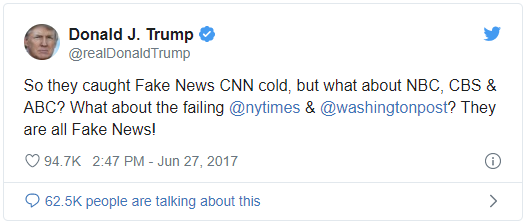
\includegraphics[width=0.7\textwidth]{./Img/Trump-Fake-News.png}
    \caption{Post udostępniony przez Donalda Trumpa na portalu Twitter}
\end{figure}

Według założonego przez dziewięć organizacji w skład których wchodzą 
Google, Facebook oraz Twitter projektu ``First Draft News''
możemy wyróżnić siedem typów Fake Newsów~\cite{TypesOfFakeNews}:
\begin{enumerate}
    \item Satyra bądź parodia - nie ma na celu wyrządzić krzywdy ale może oszukać
    \item Fałszywe połączenie - nagłowki oraz obrazy nie mają powiązania z zawartością
    \item Myląca zawartość - tekst napisany w mylący sposób
    \item Fałszywy kontekst - prawdziwa zawartość powiązana ze złym kontekstem
    \item Oszukana zawartość - źródła pochodzenia informacji są fałszywe
    \item Zmanipulowana zawartość - prawdziwa zawartość zmanipulowana w odpowiedni sposób by oszukać odbiorcę
    \item Sfabrykowana zawartość - całkowicie zmyślona zawartość mająca na celu wyrządzić krzywdę
\end{enumerate}
Jak podaje słownik ``Merriam Webster'' po raz pierwszy wykorzystano zwrot
``Fake news'' w roku 1890.


Jednym z najsłynniejszych typów fake newsów jest propaganda, czyli według 
definicji ``technika sterowania poglądami i zachowaniami ludzi polegająca na 
celowym, natarczywym, połączonym z manipulacją oddziaływaniu na zbiorowość''~\cite{SJP}
pomimo iż najczęsciej propaganda ma charakter polityczny nie jest to jedyne 
jej zastosowanie. Najstarszym przykładem pisemnej propagandy są opisy podbojów
Dariusza Wielkiego datowane na rok 515 p.n.e. Od tego czasu w historii ludzkości
można znaleźć wiele przypadków wykorzystania tego typu dezinformacji w takich krajach
jak Starożytny Rzym, Niemcy podczas drugiej wojny światowej a nawet w dzisiejszych 
czasach Korea Północna.
Propagandę można podzielić na 3 różne typy:
\begin{enumerate}
    \item Biała propaganda - źródło pochodzenia informacji jest prawdziwe i podane
    \item Szara propaganda - źródło pochodzenia informacji jest dla odbiorcy nieznane i może się on jedynie domyślać
    \item Czarna propaganda - źródło pochodzenia informacji jest umyślnie sfałszowane w celu wyrządzenia szkody 
\end{enumerate}


% historia fake newsow 
\section{Sposoby rozprzestrzeniania fałszywych informacji}
Wraz ze zmianami w sposobach rozprzestrzeniania informacji na świecie zmieniało się
także podejście do tworzenia fake newsów w odpowiedni sposób oszukujących osoby do których 
były one skierowane. 

\subsection{Gazety}
Wykorzystanie fake newsów w gazetach miało głownie na celu przyciągnąć uwage a co za 
tym idzie zwiększyć sprzedaż danej gazety. Stało się to na tyle popularne że spowodowało
narodziny nowego pojęcia ``żółtej prasy'' była to prasa starająca się z całych sił zwrocić
uwagę przechodnia poświęcając swoją wiarygodność poprzez zawarcie w nagłowkach w pełni lub
częściowo nieprawdziwych wiadomości. Dziennikarz Frank Luther Mott wyróżnia 5 cech charakteryzujących 
żółtą prasę ~\cite{YellowPressFrank}:
\begin{itemize}
    \item Napisane dużą czcionką straszące nagłówki na temat mniej ważnych wydarzeń
    \item Nadmierna ilość zdjęć i rysunków
    \item Zawarcie sfałszowanych wywiadów, mylących nagłowków, pseudonauki oraz nieprawdziwych informacji od ludzi podających się za ekspertów
    \item Dodanie w pełni kolorowych dodatków do gazet w niedzielę
    \item Stawianie siebie jako słabszego w walce przeciwko systemowi
\end{itemize}

\begin{figure}[h!]
    \centering
    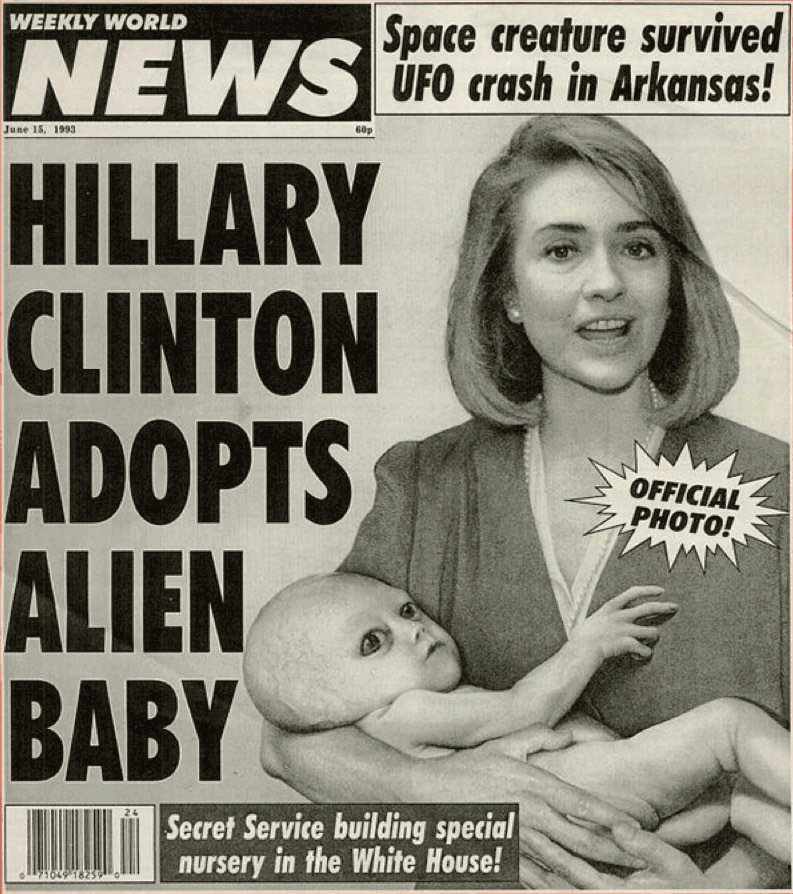
\includegraphics[width=0.5\textwidth]{./Img/fake-newspaper.jpg}
    \caption{Przykład żółtej prasy z roku 1993}
\end{figure}

\subsection{Telewizja}
Wynalezienie telewizji na początku 20 wieku zmieniło całkowicie sposób w jaki ludzie pozyskiwali wiadomości ze świata.
Aby pozyskać informacje na temat najnowszych wydarzeń nie było potrzebne kupienie gazety a nawet 
wyjście z domu, w tym celu wystarczyło posiadanie telewizji i jej uruchomienie. Połączenie zarówno obrazu
jak i dzwięku zmusiło osoby chcące oszukać swoich odbiorów do stworzenia nowych technik 
pozwalających w wiarygodny sposób przedstawić kłamstwo.

Przykładem osoby, która w znakomity sposób wykorzystała siłę daną mu przez telewizję był Edward Bernays
nazywany ``Ojcem public relations''.
W roku 1929 został on zatrudniony aby wypromować papierosy firmy ``Lucky Strike''
stworzona przez niego reklama ukazywała kobiety maszerujące ulicami Nowego Yorku
podczas palenia papierosów. Ponieważ kobiety palące były uznawane w tamtych czasach tematem
taboo autor reklamy nazwał ją w gazetach walką o prawa kobiet. Reklama ta spowodowała tak duże 
spopularyzowanie palenia papierosów, że własnie Edwardowi Bernays głownie przypisuje
ich dużą sprzedaż przez kolejne lata.
Był on także osobą dzięki której w dzisiejszych czasach diamenty są uznawane za symbol miłości po tym jak
został zatrudniony do wypromowania diamentów firmy ``De Beers''~\cite{MarkDice}.

\subsection{Internet}
Pojawienie się internetu wpłynęło na każdy element życia codziennego czynności takie jak komunikacja, rozrywka,
a także rozprzestrzenianie informacji uległy zmianom tak wielkim, że ciężko wyobrazić sobie w jaki sposób działały
one wcześniej. 

Dzięki pojawieniu się takich portali społecznościowych jak Facebook, Twitter oraz Instagram każdy użytkownik
internetu może opowiedzieć o swoich przemyśleniach, wydarzeniach z życia każdej osobie zainteresowanej. Portale te
pozwoliły nie tylko na przekazywanie informacji o sobie ale także opowiadanie o wydarzeniach ze świata przez wszystkie
chętne osoby. Wraz z rozwojem internetu stopniowo zwiększa się ilość osób czerpiących informacje na temat wydarzeń
właśnie z portali społecznościowych i do dnia dzisiejszego w Ameryce wynosi 68\% dorosłych osób. 

Udostępnienie każdej osobie możliwości wypowiedzenia się doprowadziło do sytuacji w której duża część informacji w internecie
jest całkowicie fałszywa bądź w pewien sposób zmanipulowana poprzez osobę nieobiektywnie opisującą wydarzenia. Ogrom informacji
można zauważyć na podstawie ilości potwierdzonych fake newsów związanych z wydarzeniami wokół wirusa COVID-19, których do 
20-06-2020 jest aż 110 niektóre z nich to~\cite{Korona}:
\begin{itemize}
    \item Szczepionka na koronawirusa jest ukrywana od marca
    \item Aspiryna jest lekarstwem na COVID-19
    \item Komary przenoszą koronawirusa
    \item Kraje bez sieci 5G są wolne od koronawirusa 
    \item Koronawirus nie zagraża uczestnikom zgromadzeń religijnych
    \item Koronawirus to środek do zmniejszenia populacji Ziemi
\end{itemize}
Osoby oszukane fake newsami grają istotną role w dalszym ich rozprzestrzenianiu poprzez udostępnianie informacji swoim znajomym 
lub rozmowy jest to cecha internetu, która daje niespotykaną wcześniej efektywność oszukiwania dużej ilości ludzi w szybkim
czasie. 
\begin{figure}[h!]
    \centering
    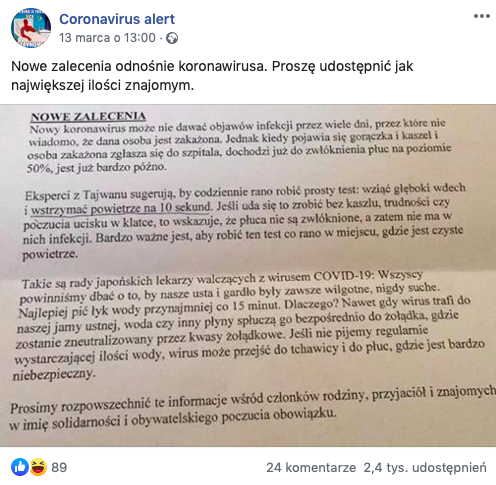
\includegraphics[width=0.7\textwidth]{./Img/cvfakenews.png}
    \caption{Przykład fałszywej informacji na portalu facebook}
\end{figure}

Na powyższym obrazie ukazany jest post udostępniony na portalu Facebook z którego wynika, że jeżeli osoba jest w stanie wstrzymać 
oddech na 10 sekund to nie jest ona zarażona na koronawirusa. Metoda ta według opisu miała być skuteczna według ekspertów 
z Japonii. Jak się później okazało informacja ta była całkowicie fałszywa nie powstrzymało to jednak ponad 2.4 tysiąca ludzi przed 
udostępnieniem jej swoim znajomym.~\cite{KoronaOddech} 

\section{Sposoby ochrony przed nieprawdziwymi informacjami}
Rozwój tak potężnego narzędzia jak internet spowodował że fałszywe informacje
stały się poważnym zagrożeniem  w dzisiejszym świecie. Aby zapobiec oszukaniu 
dużej ilości społeczeństwa znaleziono różne sposoby na ochronę przed nieprawdziwymi
informacjami niektóre z nich to 
\begin{enumerate}
    \item IFLA ``How to spot fake news''- jest to stworzona przez międzynarodową instytucję
    reprezentującą interesy bibliotekarzy i pracowników informacji o nazwie IFLA infografika
    przedstawiające listę rzeczy, które należy zrobić podejrzewając że jesteśmy oszukiwani.

    \begin{figure}[h!]
        \centering
        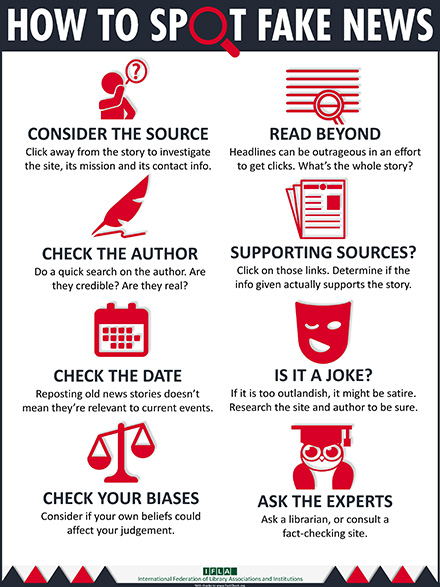
\includegraphics[width=0.5\textwidth]{./Img/how-to-spot-fake-news.jpg}
        \caption{Infografika stworzona przez IFLA}
    \end{figure}

    Czynności które są na niej zawarte to 
    \begin{itemize}
        \item Sprawdzenie źródła informacji
        \item Dokładne przeczytanie treści
        \item Sprawdzenie autora
        \item Analiza odnośników 
        \item Sprawdzenie dat związanych 
        \item Upewnienie się że informacja nie jest formą żartu
        \item Obiektywna ocena informacji
        \item Zapytanie ekspertów
    \end{itemize}
    \item Strony internetowe stworzone w celu walki z dezinformacją - istnieje
    wiele witryn gdzie eksperci sprawdzają nadesłane przez użytkowników informacje
    pod względem ich zgodności z prawdą.
    Przykładami takich portali są: \emph{fakenews.pl, snopes.com, FactCheck.org, factchecker.in} 
    \item Grupy osób powołanych przez rząd do walki z fałszywymi informacjami - najlepszym przykładem
    takiej grupy są tzw. \emph{Litewskie Elfy} jest to grupa ochotników, którzy w wolnym czasie przeglądają 
    fora internetowe oraz media społecznościowe sprawdzając znajdujące się na nich informacje. W przypadku
    znalezienia nieprawdziwej informacji osoby te informują administratora strony o problemie co najczęsciej
    prowadzi do jego rozwiązania. Nazwa grupy wzięła się z faktu że walczą oni z 
    grupami powszechnie zwanymi \emph{trollami}. Grupa ta zyskała na popularności
    w takim stopniu że rozpoczęto organizację kolejnych oddziałow w innych krajach
    między innymi na Łotwie.~\cite{Elves}
\end{enumerate}
Pomimo istnienia wielu sposobów ochrony przed fałszywymi informacjami ich ilość powoduje,
że bardzo łatwo zostać oszukanym. Z tego powodu bardzo pomocne byłoby stworzenie oprogramowania
pozwalającego na automatyczne rozpoznanie czy informacja jest prawdziwa.
Implementacja takiego systemu w mediach społecznościowych jak \emph{facebook, twitter} pozwoliłoby na usunięcie 
kłamstw zanim trafiłyby one przed oczy użytkowników. Popularne w ostatnich czasach algorytmy uczenia
maszynowego \emph{ML} oraz analizy języka naturalnego \emph{NLP} osiągają zaskakująco dobrą 
efektywność w klasyfikacji róznego rodzaju tekstów więc ich wykorzystanie w rozwiązaniu takiego 
problemu mogłoby pozwolić na rozwiązanie go albo zmniejszenie.

\section{Deep fake}
